\documentclass{beamer}

\usepackage[ruled]{algorithm2e}
\SetKw{KwRet}{return}
\usepackage{amsmath}
\usepackage{array}

\usetheme{AnnArbor}
\usecolortheme{crane}
\usefonttheme[onlymath]{serif}

\title{Deep Learning - Foundations and Concepts}
\subtitle{Chapter 13. Graph Neural Networks}
\author{nonlineark@github}
\date{\today}

\begin{document}

\begin{frame}
    \titlepage
\end{frame}

\begin{frame}
    \frametitle{Outline}
    \tableofcontents
\end{frame}

\section{Machine Learning on Graphs}

\begin{frame}
    \frametitle{Machine learning on graphs}
    There are many kinds of applications that we might wish to address using graph-structured data:
    \begin{itemize}
        \item Node prediction: Classify documents according to their topic based on the hyperlinks and citations between the documents.
        \item Edge prediction (graph completion): Knowing some of the interactions in a protein network and predict the presence of any additional ones.
        \item Graph prediction: Predict whether a particular molecule is soluble in water.
    \end{itemize}
\end{frame}

\begin{frame}
    \frametitle{Graph properties}
    \begin{itemize}
        \item A graph $\mathcal{G}=(\mathcal{V},\mathcal{E})$ consists of a set of nodes or vertices, denoted by $\mathcal{V}$, along with a set of edges or links, denoted by $\mathcal{E}$.
        \item We index the nodes by $n=1,\hdots,N$, and we write the edge from node $n$ to node $m$ as $(n,m)$.
        \item If two nodes are linked by an edge they are called neighbors, and the set of all neighbors of node $n$ is denoted by $\mathcal{N}(n)$.
        \item For each node $n$ we can represent the corresponding node variables as a $D$-dimensional column vector $x_{n}$ and we can group these into a data matrix $X$ of dimensionality $N\times{}D$.
    \end{itemize}
\end{frame}

\begin{frame}
    \frametitle{Adjacency matrix}
    A convenient way to specify the edges in a graph is to use an adjacency matrix denoted by $A$:
    \begin{itemize}
        \item To define the adjacency matrix we first have to choose an ordering for the nodes.
        \item The adjacency matrix has dimensions $N\times{}N$ and contains a $1$ in every location $n,m$ for which there is an edge going from node $n$ to node $m$, with all other entries being $0$.
        \item We could consider using adjacency matrix directly as the input to a neural network. To do this we could flatten the matrix, for example by concatenating the columns into one long column vector.
        \item The node ordering invariance should be treated as an inductive bias when constructing a network architecture.
    \end{itemize}
\end{frame}

\begin{frame}
    \frametitle{Permutation equivariance}
    \begin{itemize}
        \item A permutation $\pi$ is a bijection from $\{1,\hdots,N\}$ to itself.
        \item Let $\{e_{1},\hdots,e_{N}\}$ be the standard basis of $\mathbb{R}^{N}$, given a permutation $\pi$, the corresponding permutation matrix $P$ is defined as: $P=\begin{pmatrix}
            e_{\pi(1)}&\hdots&e_{\pi(N)}
        \end{pmatrix}^{T}$
        \item When we reorder the labelling on the nodes of a graph:
        \begin{itemize}
            \item The data matrix $X$ is changed to $\tilde{X}=P^{T}X$.
            \item The adjacency matrix $A$ is changed to $\tilde{A}=P^{T}AP$.
            \item Any global property of the graph does not depend on node label reordering: $y(\tilde{X},\tilde{A})=y(X,A)$.
            \item Node predictions should be equivariant with respect to node label reordering: $y(\tilde{X},\tilde{A})=P^{T}y(X,A)$.
        \end{itemize}
    \end{itemize}
\end{frame}

\section{Neural Message-Passing}

\begin{frame}
    \frametitle{Convolutional filters}
    Consider a convolutional layer using $3\times{}3$ filters. The computation performed by a single filter at a single pixel in layer $l+1$ can be expressed as:
    \begin{equation*}
        z^{(l+1)}_{i}=f(\sum_{j}w_{j}z^{(l)}_{j}+b)
    \end{equation*}
    This is not equivariant under reordering of the nodes in layer $l$. However, we can achieve equivariance with some simple modifications as follows:
    \begin{equation*}
        z^{(l+1)}_{i}=f(w_{\textrm{neigh}}\sum_{j\in\mathcal{N}(i)}z^{(l)}_{j}+w_{\textrm{self}}z^{(l)}_{i}+b)
    \end{equation*}
    where a single weight parameter $w_{\textrm{neigh}}$ is shared across the neighbors, and node $i$ has its own weight parameter $w_{\textrm{self}}$.
\end{frame}

\begin{frame}
    \frametitle{Convolutional filters}
    \begin{figure}
        \caption{A convolutional filter for images can be represented as a graph-structured computation}
        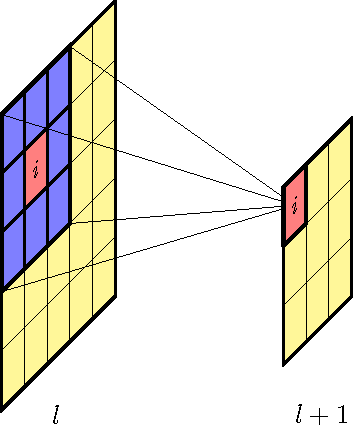
\includegraphics[height=0.6\textheight,trim=0 0 -1cm 0]{Figure_3_a.pdf}
        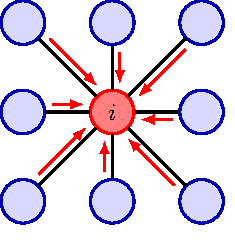
\includegraphics[trim=-1cm 0 0 0]{Figure_3_b.pdf}
    \end{figure}
\end{frame}

\begin{frame}
    \frametitle{Graph convolutional networks}
    We can view each layer of processing as having two successive stages:
    \begin{itemize}
        \item Aggregation stage: For each node $n$, messages are passed to that node from its neighbors and combined to form a new vector $z^{(l)}_{n}$ in a way that is permutation invariant: $z^{(l)}_{n}=\mathrm{Aggregate}(\{h^{(l)}_{m}:m\in\mathcal{N}(n)\})$.
        \item Update stage: The aggregated information from neighboring nodes is combined with local information from the node itself and used to calculate a revised embedding vector for that node: $h^{(l+1)}_{n}=\mathrm{Update}(h^{(l)}_{n},z^{(l)}_{n})$.
    \end{itemize}
\end{frame}

\begin{frame}
    \frametitle{Graph convolutional networks}
    \begin{algorithm}[H]
        \caption{Simple message-passing neural network}
        \For{$l\gets{}0$ \KwTo $L-1$}{
            $z^{(l)}_{n}\gets\mathrm{Aggregate}(\{h^{(l)}_{m}:m\in\mathcal{N}(n)\})$\;
            $h^{(l+1)}_{n}\gets\mathrm{Update}(h^{(l)}_{n},z^{(l)}_{n})$\;
        }
        \Return{$\{h^{(L)}_{n}\}$}\;
    \end{algorithm}
\end{frame}

\begin{frame}
    \frametitle{Aggregation operators}
    Some simple aggregation functions:
    \begin{align*}
        \mathrm{Aggregate}(\{h^{(l)}_{m}:m\in\mathcal{N}(n)\})&=\sum_{m\in\mathcal{N}(n)}h^{(l)}_{m} \\
        \mathrm{Aggregate}(\{h^{(l)}_{m}:m\in\mathcal{N}(n)\})&=\frac{1}{|\mathcal{N}(n)|}\sum_{m\in\mathcal{N}(n)}h^{(l)}_{m} \\
        \mathrm{Aggregate}(\{h^{(l)}_{m}:m\in\mathcal{N}(n)\})&=\sum_{m\in\mathcal{N}(n)}\frac{h^{(l)}_{m}}{\sqrt{|\mathcal{N}(n)||\mathcal{N}(m)|}} \\
        \mathrm{Aggregate}(\{h^{(l)}_{m}:m\in\mathcal{N}(n)\})&=\max(\{h^{(l)}_{m}:m\in\mathcal{N}(n)\})
    \end{align*}
\end{frame}

\begin{frame}
    \frametitle{Aggregation operators}
    We can introduce learnable parameters by:
    \begin{itemize}
        \item First transforming each of the embedding vectors from neighboring nodes using a multilayer neural network, denoted by $\mathrm{MLP}_{\phi}$.
        \item Then transforming the combined vector with another neural network $\mathrm{MLP}_{\theta}$.
    \end{itemize}
    to give an overall aggregation operator:
    \begin{equation*}
        \mathrm{Aggregate}(\{h^{(l)}_{m}:m\in\mathcal{N}(n)\})=\mathrm{MLP}_{\theta}(\sum_{m\in\mathcal{N}(n)}\mathrm{MLP}_{\phi}(h^{(l)}_{m}))
    \end{equation*}
    in which $\mathrm{MLP}_{\phi}$ and $\mathrm{MLP}_{\theta}$ are shared across layer $l$.
\end{frame}

\begin{frame}
    \frametitle{Update operators}
    A simple form for the update operator would be:
    \begin{equation*}
        \mathrm{Update}(h^{(l)}_{n},z^{(l)}_{n})=f(W_{\textrm{self}}h^{(l)}_{n}+W_{\textrm{neigh}}z^{(l)}_{n}+b)
    \end{equation*}
    If we choose a simple summation as the aggregation function and if we also share the same weight matrix between nodes and their neighbors, we obtain a particularly simple form of the update operator:
    \begin{equation*}
        h^{(l+1)}_{n}=\mathrm{Update}(h^{(l)}_{n},z^{(l)}_{n})=f(W^{(l+1)}\sum_{m\in\mathcal{N}(n),n}h^{(l)}_{m}+b)
    \end{equation*}
\end{frame}

\begin{frame}
    \frametitle{Node classification}
    We need to define a cost function for training:
    \begin{itemize}
        \item For node classification over $C$ classes, we can use $\mathrm{softmax}(H^{(L)}_{n}W^{(o)})$ to output the logits, where $W^{(o)}$ is a learnable $D\times{}C$ matrix. The loss function is defined as the cross-entropy loss across all nodes and all classes.
        \item If the goal is to predict continuous values at the outputs then a simple linear transformation can be combined with a sum-of-squares error to define a suitable loss function.
    \end{itemize}
\end{frame}

\begin{frame}
    \frametitle{Node classification}
    We can distinguish between three types of nodes as follows:
    \bigbreak
    \begin{tabular}{m{15em}|m{3em} m{3em} m{3em}}
        &$\mathcal{V}_{\textrm{train}}$&$\mathcal{V}_{\textrm{trans}}$&$\mathcal{V}_{\textrm{induct}}$ \\
        \hline
        Labelled&Yes&No&No \\
        \hline
        Included in the message-passing operations of the graph neural network&Yes&Yes&No \\
        \hline
        Used to compute the loss function used for training&Yes&No&No
    \end{tabular}
    \bigbreak
    If there are no transductive nodes, then the training is generally referred to as inductive learning. However, if there are transductive nodes then it is called transductive learning.
\end{frame}

\begin{frame}
    \frametitle{Edge classification}
    A common form of edge classification task is edge completion in which the goal is to determine whether an edge should be present between two nodes. The probability $p(n,m)$ for the presence of an edge between nodes $n$ and $m$ can be defined as:
    \begin{equation*}
        p(n,m)=\sigma(h_{n}^{T}h_{m})
    \end{equation*}
\end{frame}

\begin{frame}
    \frametitle{Graph classification}
    In some applications of graph neural networks, the goal is to predict the properties of new graphs given a training set of labelled graphs $\mathcal{G}_{1},\hdots,\mathcal{G}_{N}$. This requires that we combine all the final-layer embedding vectors in a way that does not depend on the arbitrary node ordering:
    \begin{equation*}
        y=f(\sum_{n\in\mathcal{V}}h^{(L)}_{n})
    \end{equation*}
    where the function $f$ may contain learnable parameters. Other invariant aggregation functions can be used such as averages or element-wise minimum or maximum.
\end{frame}

\section{General Graph Networks}

\begin{frame}
    \frametitle{Graph attention networks}
    Graph attention networks can capture an inductive bias that says some neighboring nodes will be more important than others in determining the best update in a way that depends on the data itself:
    \begin{equation*}
        z^{(l)}_{n}=\mathrm{Aggregate}(\{h^{(l)}_{m}:m\in\mathcal{N}(n)\})=\sum_{m\in\mathcal{N}(n)}A_{nm}h^{(l)}_{m}
    \end{equation*}
    where the attention coefficients $A_{nm}$ should satisfy:
    \begin{align*}
        A_{nm}&\ge{}0 \\
        \sum_{m\in\mathcal{N}(n)}A_{nm}&=1
    \end{align*}
\end{frame}

\begin{frame}
    \frametitle{Graph attention networks}
    Some ways to construct the attention coefficients:
    \begin{equation*}
        A_{nm}=\frac{\exp(h_{n}^{T}Wh_{m})}{\sum_{m'\in\mathcal{N}(n)}\exp(h_{n}^{T}Wh_{m'})}
    \end{equation*}
    where $W$ is a $D\times{}D$ matrix of learnable parameters. Or:
    \begin{equation*}
        A_{nm}=\frac{\exp(\mathrm{MLP}(h_{n},h_{m}))}{\sum_{m'\in\mathcal{N}(n)}\mathrm{MLP}(h_{n},h_{m'})}
    \end{equation*}
    where the $\mathrm{MLP}$ has a single continuous output variable whose value is invariant if the input vectors are exchanged.
\end{frame}

\begin{frame}
    \frametitle{Edge embeddings}
    Some networks also have data associated with the edges. In addition to the node embeddings given by $h^{(l)}_{n}$, we therefore introduce edge embeddings $e^{(l)}_{nm}$. We can then define general message-passing equations in the form:
    \begin{align*}
        e^{(l+1)}_{nm}&=\mathrm{Update}_{\textrm{edge}}(e^{(l)}_{nm},h^{(l)}_{n},h^{(l)}_{m}) \\
        z^{(l+1)}_{n}&=\mathrm{Aggregate}_{\textrm{node}}(\{e^{(l+1)}_{nm}:m\in\mathcal{N}(n)\}) \\
        h^{(l+1)}_{n}&=\mathrm{Update}_{\textrm{node}}(h^{(l)}_{n},z^{(l+1)}_{n})
    \end{align*}
\end{frame}

\begin{frame}
    \frametitle{Graph embeddings}
    In addition to node and edge embeddings we can also maintain and update an embedding vector $g^{(l)}$ that relates to the graph as a whole. We can define general message-passing equations:
    \begin{align*}
        e^{(l+1)}_{nm}&=\mathrm{Update}_{\textrm{edge}}(e^{(l)}_{nm},h^{(l)}_{n},h^{(l)}_{m},g^{(l)}) \\
        z^{(l+1)}_{n}&=\mathrm{Aggregate}_{\textrm{node}}(\{e^{(l+1)}_{nm}:m\in\mathcal{N}(n)\}) \\
        h^{(l+1)}_{n}&=\mathrm{Update}_{\textrm{node}}(h^{(l)}_{n},z^{(l+1)}_{n},g^{(l)}) \\
        g^{(l+1)}&=\mathrm{Update}_{\textrm{graph}}(g^{(l)},\{h^{(l+1)}_{n}:n\in\mathcal{V}\},\{e^{(l+1)}_{nm}:(n,m)\in\mathcal{E}\})
    \end{align*}
\end{frame}

\begin{frame}
    \frametitle{Graph embeddings}
    \begin{algorithm}[H]
        \caption{Graph neural network with node, edge, and graph embeddings}
        \For{$l\gets{}0$ \KwTo $L-1$}{
            $e^{(l+1)}_{nm}\gets\mathrm{Update}_{\textrm{edge}}(e^{(l)}_{nm},h^{(l)}_{n},h^{(l)}_{m},g^{(l)})$\;
            $z^{(l+1)}_{n}\gets\mathrm{Aggregate}_{\textrm{node}}(\{e^{(l+1)}_{nm}:m\in\mathcal{N}(n)\})$\;
            $h^{(l+1)}_{n}\gets\mathrm{Update}_{\textrm{node}}(h^{(l)}_{n},z^{(l+1)}_{n},g^{(l)})$\;
            $g^{(l+1)}\gets\mathrm{Update}_{\textrm{graph}}(g^{(l)},\{h^{(l+1)}_{n}:n\in\mathcal{V}\},\{e^{(l+1)}_{nm}:(n,m)\in\mathcal{E}\})$\;
        }
        \Return{$\{h^{(L)}_{n}\}$,$\{e^{(L)}_{nm}\}$,$g^{(L)}$}\;
    \end{algorithm}
\end{frame}

\begin{frame}
    \frametitle{Over-smoothing}
    One significant problem that can arise with some graph neural networks is called over-smoothing in which the node-embedding vectors tend to become very similar to each other after a number of iterations of message-passing. One way to help alleviate this issue is to introduce residual connections:
    \begin{equation*}
        h^{(l+1)}_{n}=\mathrm{Update}_{\textrm{node}}(h^{(l)}_{n},z^{(l+1)}_{n},g^{(l)})+h^{(l)}_{n}
    \end{equation*}
    Another approach for mitigating the effects of over-smoothing is to allow the output layer to take information from all previous layers of the network and not just the final convolutional layer:
    \begin{equation*}
        y_{n}=f(h^{(1)}_{n}\oplus\hdots\oplus{}h^{(L)}_{n})
    \end{equation*}
    where $a\oplus{}b$ denotes the concatenation or max pooling of vectors $a$ and $b$.
\end{frame}

\begin{frame}
    \frametitle{Regularization}
    \begin{itemize}
        \item Standard techniques: For example, adding the sum-of-squares of the parameter values to the loss function.
        \item Parameter sharing: Weights and biases can also be shared across layers to reduce the number of independent parameters.
        \item Dropout: Omitting random subsets of the graph nodes or edges during training.
    \end{itemize}
\end{frame}

\begin{frame}
    \frametitle{Geometric deep learning}
    In applications of graph neural networks associated with spatial properties, there are additional equivariance and invariance properties that can be built into the network architecture. For example, the task of predicting the properties of a molecule:
    \begin{itemize}
        \item The molecule can be represented as a list of atoms of given types along with the spatial coordinates of each atom denoted by $r^{(l)}_{n}$.
        \item The values for $r^{(l)}_{n}$ depends on the arbitrary choice of coordinate system, whereas the properties of the molecule do not:
        \begin{itemize}
            \item Translation.
            \item Rotation.
            \item Reflection.
        \end{itemize}
    \end{itemize}
\end{frame}

\begin{frame}
    \frametitle{Geometric deep learning}
    The new embeddings $r^{(l)}_{n}$ can be incorporated into the graph neural network update equations to achieve the required symmetry properties:
    \begin{align*}
        e^{(l+1)}_{nm}&=\mathrm{Update}_{\textrm{edge}}(e^{(l)}_{nm},h^{(l)}_{n},h^{(l)}_{m},||r^{(l)}_{n}-r^{(l)}_{m}||^{2}) \\
        r^{(l+1)}_{n}&=r^{(l)}_{n}+C\sum_{m\in\mathcal{N}(n)}(r^{(l)}_{n}-r^{(l)}_{m})\phi(e^{(l+1)}_{nm}) \\
        z^{(l+1)}_{n}&=\mathrm{Aggregate}_{\textrm{node}}(\{e^{(l+1)}_{nm}:m\in\mathcal{N}(n)\}) \\
        h^{(l+1)}_{n}&=\mathrm{Update}_{\textrm{node}}(h^{(l)}_{n},z^{(l+1)}_{n})
    \end{align*}
    where $\phi$ is a general scalar function of the edge embeddings and is represented by a neural network, and the coefficient $C$ is typically set equal to the reciprocal of the number of terms in the sum.
\end{frame}

\end{document}